\documentclass[12pt]{article}
\usepackage[english]{babel}
\usepackage[utf8x]{inputenc}
\usepackage{amsmath}
\usepackage{graphicx}

\begin{document}
\begin{titlepage}

% definition of custom command for horizontal lines
\newcommand{\HRule}{\rule{\linewidth}{0.5mm}}

\center
% HEADING
\textsc{\LARGE University of Dublin,\\Trinity College}\\[1.0cm]

\includegraphics[width=0.2\textwidth]{logo.png}

\HRule \\[0.4cm]
\textsc{\Large Dice Investigation}\\[0.25cm]
\textsc{\large ST2004 \& ST2353 Assessment 1}\\[0.1cm]
\HRule \\[0.4cm]
 
% AUTHORS
\begin{minipage}{0.5\textwidth}
\begin{flushleft} \large
\emph{Authors:}
\\Alexandru \textsc{Sulea} 12315152
\\Edmond \textsc{O'Flynn} 12304742
\\Jonathan \textsc{Lester} 12345678
\\Ronan \textsc{Campbell} 12345678
\end{flushleft}
\end{minipage}
~
\begin{minipage}{0.4\textwidth}
\begin{flushleft} 
\large
\emph{Lecturer:} \\
Dr. Brett \textsc{Houlding}
\vspace{1.9cm}
\end{flushleft}
\end{minipage}\\[2cm]

% DATE
{\large \today}\\[1cm] 

% LOGO
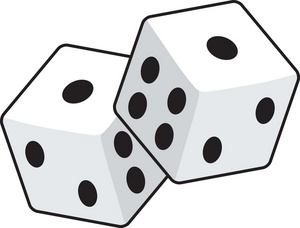
\includegraphics[width=0.3\textwidth]{dice.png}
\clearpage

\end{titlepage}

\tableofcontents
\listoffigures
\addcontentsline{toc}{section}{List of Figures}
\listoftables
\addcontentsline{toc}{section}{List of Tables}

\addcontentsline{toc}{section}{References}

\thispagestyle{empty}
\cleardoublepage
\setcounter{page}{1}

\section{q1i}
Q1i
\clearpage

\section{Q1ii: Probability Distributions}
\subsection{Permutation}
Three dice can be rolled in a variety of 216 ways (6*6*6) over a probability distribution shown above in fig x.x. The possible combinations for each die results in varied probabilities for each number, where a greater number of combinations results in a higher probabilistic outcome, and thus over the long run, results in a variance of probabilities for each dice combination. The probability of each number rolled tends from the value of the number of combinations that can be possibly formed for that combination, with respect to the total number of combinations possible for n dice.\\
Expected value is defined as the product of given value with respect to thte probabilistic outcome of that value, as a summation of all the possible values  within that set for a randomly distributed variable X:\\
$$E[X_n]=x_np_n$$
$$E[X]=\sum_{i}^{n}x_np_n$$\\
Given the probability distribution, the expected value is calculated as such:
$$E[X]=1*\frac{1}{6}+1*\frac{2}{6}+1*\frac{3}{6}+1*\frac{4}{6}+1*\frac{5}{6}+1*\frac{6}{6}=3.5$$
In the case of having three dice, this method can be extended to encapsulate a wider range of values over two additional dice:\\
$$E[X]=3*\frac{1}{216}+4*\frac{3}{216}+5*\frac{6}{216}+6*\frac{10}{216}+7*\frac{15}{216}+8*\frac{21}{216}+9*\frac{25}{216}+10*\frac{27}{216}+$$\\$$11*\frac{27}{216}+12*\frac{25}{216}+13*\frac{21}{216}+14*\frac{15}{216}+15*\frac{10}{216}+16*\frac{6}{216}+17*\frac{3}{216}+18*\frac{1}{216}$$\\
The rolling of dice in such a way is denoted as an independent event, as the dice rolls in the future are not dependent on previous rolls and do not affect the outcome of values, where essentially the expected outcome of the event is given by:\\
$$E[X+Y+Z]=E[X]+E[Y]+E[Z]$$\\
Given the independence of each die roll, the expected value for three rolls is given by:\\
$$E[X+Y+Z]=3.5+3.5+3.5+3.5$$\\

\subsection{graphs}
\clearpage

\section{q1iii}
Q1iii
\clearpage

\section{q2}
Q2
\clearpage

\end{document}
